% \begin{savequote}[75mm]
% Nulla facilisi. In vel sem. Morbi id urna in diam dignissim feugiat. Proin molestie tortor eu velit. Aliquam erat volutpat. Nullam ultrices, diam tempus vulputate egestas, eros pede varius leo.
% \qauthor{Quoteauthor Lastname}
% \end{savequote}

\chapter{Object representations in lateral visual cortex}
\newthought{Shape is a diagnostic feature} of object identity. Visually similar objects, such as a pear and an apple, can be grouped together by certain shared visual features. On the other hand, different images or views of any one object can look dramatically dissimilar, yet still belong to the same object (REFREF example?). In the first chapter, we established the behavioral ability of rats to perform visual object recognition and quantified their perceptual choices of object similarity. We next turned our attention to the neuronal substrates of these abilities. 

% Neural subtrates of object recog. -- what do we know from primates.
In the primate brain, the ventral visual pathway is thought to transform non-diagnostic, low-level representations of features that may be common to many different objects into high-level representations that are both diagnostic of object identity, or selective for a given object, and robust to variations in particular appearance, or tolerant to identity-preserving transformations. 

Primate visual cortex is arranged hierarchically, with visual inputs from the thalamus first arriving in so-called ``striate'' cortex (also known as area V1), before being processed and forwarded through a successive chain of hierarchically-organized visual areas (area V2 > area V4 > inferotemporal cortex) curving along the ventral surface of the brain. Along each stage of the ventral stream, there is a gradual increase in object selectivity and tolerance, culminating in area IT, at the highest level of the ventral pathway. 

Several key trends have been observed in the response properties of visual neurons as one progresses from ``lower'' to ``higher'' visual areas along this ventral pathway. First, the region of visual space that a given cell responds to (the ``receptive field'') gradually increases as one moves along the ventral pathway, with receptive fields in the highest stages of visual cortex sometimes responding to up to half of the visual field\cite{op2000spatial}. Meanwhile, selectivity for complex object features also increases along the ventral visual pathway, with neurons in later stages of the pathway responding only to very particular configurations of features\cite{Desimone1984, Logothetis1996}.  Critically, as one progresses along the ventral pathway, neurons also exhibit greater tolerance to identity-preserving transformation of the retinal image -- that is, neurons tend to retain their selectivity for particular object features even if those features are, for instance, moved around on the retina, or scaled up or down in size\cite{Ito1995}.These combined features of selectivity and tolerance are in many ways the key computational hallmarks of high-level vision\cite{DiCarlo2007, DiCarlo2012}. 

% Previous rodent studies
\section{Lateral visual cortex exhibits some of the same core properties found in primates}
Anatomical studies have shown that the connectivity of rodent visual cortex observes a similar hierarchical pattern, with thalamic inputs arriving in an analogous striate area V1 in posterior of the brain, and then projecting ventrally to a series of interconnected extrastriate areas\cite{Coogan1993, ETC}. However, while these areas have been characterized anatomically, much less is known about their function.

Since 
% shape selectivity
% natural vs scrambled
% vs. category representations (Vinken)
% tolerance

Consistent with previous studies in rats, and what might be expected from a primate-like hierarchical organization, we observed increasing receptive field sizes in areas V1, LM, and LI (see Chapter 3). However, consistent with studies in mice, we also found asymmetries in visual field representations and motion tuning preferences that may be particular to rodent visual cortex. To determine the extent to which rat lateral visual cortex intrinsically exhibits properties thought to be important for spontaneous, as opposed to learned, object recognition behavior, we recorded from neural populations in awake, naive rats presented with a subset of the same stimuli used for the trained rats (see Chapter 1, Figure\ref{fig:behavior_generalization}) to probe axes of transformation in which object identity is either preserved or gradually morphed to a new identity across changes.


% ---------------------------------------------------------------
% Single neuron selectivity and tolerance
% ---------------------------------------------------------------
\section{Single neurons exhibit selectivity and tolerance}
One key feature of the primate ventral stream is a gradual increase in shape or object selectivity and a parallel increase in tolerance to identity-preserving transformations. Previous studies have shown that single-units in monkey IT exhibit a trade-of between these properties: neurons that are highly selective are less tolerant to identity-preserving transformations and highly tolerant neurons are not as selective to particular objects\cite{Zoccolan2007}.

To determine whether single neurons exhibited similar characteristics in rat visual areas, we first measured single neuron response profiles in areas V1, LM, and LI. For identity-changing transformations, we tested a subset of the morphs used to probe trained animals’ naive perceptual boundaries (see Figure\ref{fig:behavior_generalization}\textbf{REFREF}), and for identity-preserving transformations, we tested a subset of sizes covering the range of stimulus sizes used to test behavioral generalization to identity-preserving transformations (see Figure\ref{fig:behavior_generalization}\textbf{REFREF}). Since size changes come with large changes in luminance, we also presented a subset of full-screen gray-scale stimuli that were luminance-matched to each size tested (Figure\ref{fig:selectivity_tolerance}\textbf{A}).

\begin{figure}[t!]
    \includegraphics[width=\textwidth]{figures/chapter_4/fig_4-1_single_cell_selectivity_tolerance/fig_4-1_single_cell_selectivity_tolerance.pdf}
    \vspace{.1in}
    \caption[Selectivity and tolerance in single neurons]{Selectivity and tolerance in single neurons. 
    \textbf{A.} Experiment design:  5 stimulus sizes (green box) were used to test identity-preserving transformations, and nine morph levels (purple box) were used to test identity-changing transformations. 5 size-matched luminance stimuli (fullscreen, grayscale; orange box) were also included to control for luminance differences due to changes in size. 
    \textbf{B.} Schematic of flattened rat visual cortex highlighting the path of lateral visual areas highlighted in the current study. \textbf{C.} Morph selectivity (left) and size tolerance (right) for an example V1 FOV (see Methods). Thin, black curves denote tuning profiles for single cells. Colored lines point out individual cells whose averaged timecourses are shown for each tested condition below. Purple corresponds to the first set of traces (middle), while green corresponds to the second set of traces (bottom). Each timecourse is arranged as shown in \textbf{A}. Black lines and shading show mean and SEM across repetitions of each stimulus condition. 
    \textbf{D.} Same as \textbf{C}, but for an example LM FOV.
    \textbf{E.} Same as \textbf{B} and \textbf{C}, but for an example LI FOV.
    \textbf{F.} Distributions of size tolerance across all cells measured in areas V1, LM, and LI. Each dot is a cell, and black lines denote mean and SD across cells.
    \textbf{G.} Same as \textbf{F}, but for single cell measures of morph selectivity. 
    \textbf{H.} Correlation between size tolerance and morph selectivity for example V1 (left), LM (middle), and LI (right) FOVs. Each dot is a cell. Black line and shading, linear fit and 95\% CI.
    \label{fig:selectivity_tolerance}}
\end{figure}

All areas contained a diverse range of object selective and size tolerant cells. For example, even in one V1 FOV, we found cells that exhibited clear size tuning without morph selectivity, morph tuning that was preserved across different sizes, as well as luminance-tuned cells that were also sensitive or insensitive to the different morphs and sizes (Figure\ref{fig:example_blob_responsesREFREF}). 

Overall, we found that across our object stimuli, cells in LI had the lowest lifetime sparseness, while cells in V1 and LM were similarly high in sparseness (REFREF, stats, Mann-Whitney U Test, multiple comparisons). Since the images varied in morph level and size, the sparseness observedin V1 and LM could reflect a higher selectivity for morph shapes or a lower tolerance for varying sizes. To quantify the amount of object selectivity and tolerance, we calculated a morph selectivity index (MX) and a size tolerance index (ST) for each cell\cite{Zoccolan2007}. We found a range of tuning profiles across cells that was comparable between the three areas (Figure\ref{fig:selectivity_tolerance}B-D). On average, we found that relative to V1 and LM, LI cells were both less selective to morphs and more tolerant to size (Figure\ref{fig:selectivity_tolerance}E-F). Notably, this difference was not attributable to overall lower response magnitudes in LI: although we found fewer LI cells selective or responsive to the object stimuli overall, of the cells that were responsive, response magnitudes were comparable across areas (REFREF). 

It is possible that the relatively higher average morph selectivity in V1 and LM cells reflects greater sensitivity to overall luminance values. To characterize the extent to which size or morph tuning simply tracks luminance sensitivity, we calculate the correlation between each cell's size tuning curve and its tuning curve for the size-matched luminance stimuli (Supplemental Figure\ref{fig:supp_X}). While there were indeed cells whose size- or morph-tuning profiles were tightly correlated with broad luminance levels, this was not the case for the majority of cells (V1: 9.8+/-6.8\% of cells with significant correlation between size and luminance tuning across, n=REFREF cells across REFREF imaging sites; LM: 12.6+/-8.2\%, n=REFREF cells across REFREF imaging sites; Li: 12.2+/-9.1\%, n=REFREF cells across REFREF imaging sitse). 

To determine whether rat neurons exhibit a similar trade-off between shape selectivity and transformation tolerance, we calculated the correlation between morph selectivity and size tolerance for simultaneously recorded cells in each imaging site (Figure\ref{fig:selectivity_tolerance}\textbf{H}). We found a strong, negative correlation between morph selectivity and size tolerance for areas LM and LI (REFREF stats, Pearson’s r=REFREF, p<0.01). Notably, we also saw a negative correlation for V1 imaging sites, but to a weaker degree. To determine whether the strength of this trade-off differed between the three areas, we scrambled each cell’s selectivity index and tolerance index and compared correlation coefficients for those populations that passed the shuffle test (shuffle test, p<0.05 over 5000 iterations, REFREF). We found that correlation coefficients for sites in areas LM and LI were significantly more negative than those in area V1 (REFREF, stats, p<0.05, Mann-Whitney U Test, Bonferroni-corrected for multiple comparisons). 

% A critical property of single neurons in IT is the preservation of rank-ordered object selectivity, that is, relative tuning preference for a set of objects is maintained across changes in identity-preserving transformations such as position or size\cite{Li2009, REFREF}. 

% ---------------------------------------------------------------
% Morphs
% ---------------------------------------------------------------
\section{Single cells show object discriminability}
% Morphs -- neurometric curves, single-neuron disriminability
-For cells selective to either object A or object B, we calculated a measure of single neuron discriminability. AUC -- see paper. 


% ---------------------------------------------------------------
% Arousal
% ---------------------------------------------------------------
\section{Arousal modulates tuning properties} REFREF
-Head-fixed, so can monitor arousal with face tracking.
-Larger response magnitudes in high arousal states.
-Overall increase in selectivity (increased shape selectivity and decreased size tolerance)
-signal correlation & noise correlation for High vs. Low arousal
-also, signal correlation & noise correlation as a function of cortical distance. 

Face video was acquired simultaneously and synced with neural acquisition. Arousal states modulate both single neuron tuning and population decodability. We do not know how population representations supporting object recognition change across different arousal states. Trials were separated into “high” or “low” states by pupil size, and we compared single unit metrics of size tolerance and shape selectivity as well as linear separability of population representations across areas V1, LM and LI. 

Across all visual areas, shape selectivity was greater and size tolerance was lower in high arousal states compared to low arousal states at the level of single cells. In V1, but not in LM and LI, this resulted in a reduced steepness in slope for the linear fit of size tolerance as a function of morph selectivity. Also in V1, the strength of this relationship, as measured by the correlation coefficient between size tolerance and morph selectivity, was weaker in high arousal states. These results suggest a possible decoupling between selectivity and tolerance in V1 populations, such that increases in shape selectivity come at a lower cost of reduction in size tolerance in high arousal states, relative to low arousal states.

% ---------------------------------------------------------------
% Population responses
% ---------------------------------------------------------------
\section{Population responses are linearly separable}
How the brain achieves the critical combination of high object selectivity with high tolerance to particular views remains a mystery. It is thought that each successive stage of the ventral stream computes a series of operations that make object representations increasingly linearly separable. In our behavior experiments, rats accurately classified novel image transformations in the absence of any feedback, suggesting explicit training is not required for generalization behavior (see Figure\ref{fig:behavior_generalization}). The single neuron response properties in our naive rats suggest that rat visual cortex may have some of the important features considered to be important for tolerant visual object representations.

However, during behavior, the animal has access to much more than the activity of a single neuron. To determine the extent to which neural populations in rat visual cortex are inherently capable of representations that support discrimination and generalization, we took a population-based approach to compare areas V1, LM, and LI in awake, but untrained rats. Specifically, we trained linear SVMs with neural responses to these same object images to classify the responses as belonging to object A or object B\cite{Hung2005, Li2009, Rust2010, etc}. We then tested the classifiers on each of the two types of generalization tasks performed by the trained rats. 

Before testing the ability of each population to generalize across identity-preserving transformations, we first tested how well the objects could be discriminated from each other at each of the tested transformations. That is, if a given population failed to discriminate the objects at a given size, failure to generalize to that size would be trivial. For each imaging site, or set of simultaneously recorded cells, in each visual area, we trained linear classifiers to discriminate the two objects at each size, then scored accuracy on trials of the same condition that the classifier had never seen. To avoid trivial generalization due to poor baseline performance, only those populations with average test accuracies greater than accuracies calculated from shuffled object labels were included (p<0.05, REFREF). 

To test discriminability of the two anchor objects, we first tested neural representations under a “Train 1, test same” regime: At each stimulus size tested, we trained classifiers to discriminate object A from object B. Overall, discrimination accuracy improved with increasingly larger stimulus sizes (Figure\ref{fig:SuppREFREF}). This is consistent with previous single-unit studies of aggregated populations, though here we report performance for simultaneously recorded populations. This stimulus size dependence was present in all visual areas, and notably, overall performance was comparable across areas, as well. Specifically, average test scores were similar for populations in V1, LM, and LI, with mean scores in V1 and LM being slightly higher, but not significantly different, than LI (mean accuracy +/- std: V1, 0.73 +/- 0.08, n=9 sites; Lm: 0.68 +/- 0.04, n=5 sites; Li: -0.64 +/- 0.09, n=4 sites; Mann-Whitney U test, p>0.05 corrected for multiple comparisons). As expected, we also found better discrimination accuracy for larger neural population sizes (Figure\ref{fig:SuppREFREF}). Only imaging sites that passed this baseline discrimination task were included in further tests of generalization performance (see Methods). 

% Linear separability.
To quantify linear separability, we trained linear classifiers (support vector machines) to discriminate the two original objects from the neural responses in each area across different training regimes. The linear-readout scheme is important in that it is a simple, biologically plausible processing step that amounts to a thresholded sum taken over weighted synapses\cite{REFREF}. This classifier approach does not provide a measure for the total information present in the population, but rather estimates the lower bound on the information explicitly accessible to the population to support the visual task. 

We started with a “Train all, test all” scheme:  Classifiers were first trained to discriminate object A from object B across all stimulus conditions, then tested on new samples of object A and object B. This is a measure of how separable object representations are across the different stimulus sizes. We found that classifier accuracy was comparable across areas V1, LM, anbd LI for all population sizes (Figure\ref{fig:neural_generalization}B). % OVERLAP RFS?

% Arousal
% Increased shape selectivity could result in better linear separability, but decreased size tolerance could result in worse linear separability. REFREF.
% Arousal
% Consistent with the above results, we also found that linear separability of object representations was improved in high arousal states for V1, but was unaffected in LI, despite all areas exhibiting shifts in tolerance and selectivity in the same directions. However, LM also exhibited improved linear separability in high arousal states, like V1, despite there being no significant change in the linear relationship between selectivity and tolerance. This suggests that the tolerance/selectivity tradeoff may differentially affect object encoding and readout across visual areas.

% Generalization.
Based on the performance of our trained rats, we know that behaving animals achieve high levels of accuracy on completely novel, never-before-seen views of objects (see Figure\ref{fig:behavior_generalization}). To determine whether this might be true even in naive, untrained animals, we conducted a second test of generalization. Generalization to completely novel stimulus conditions was called the “Train 1, test each of the others” scheme:  We trained classifiers to discriminate object A from B at one stimulus size, then tested how well they generalized to each of the other, novel stimulus sizes. For example, if we test on stimulus size 10, the test cases were 1 “trained” condition (different samples of stimulus size 10), and 4 “novel” conditions (the 4 other stimulus sizes that the classifier never saw). We observed accuracies well above chance for all visual areas, with overall accuracies improving for larger population sizes (Figure\ref{fig:neural_generalization}C). 

Notably, the gap between accuracy for trained and novel conditions was smaller for LI, compare to V1 and LM. Given the earlier observation that single cells in LI exhibited a slightly higher size tolerance, we asked whether generalization performance was dependent on which stimulus sizes the classifiers had access to in training. Trivially, generalization might be better if the difference in training and testing conditions is small: training to discriminate object A from B at stimulus size 10 might result in better generalization to stimulus size 20, compared to generalization to stimulus size 50. For each visual area, we calculated a generalization score, defined as the ratio of accuracy on trained conditions versus novel conditions. Since a high generalization score is trivially possibly for poor performance on both trained and novel conditions, we calculated this metric only for the largest, that is, best-performing population sizes for each visual area (n=128 cells). As expected, we found that generalization was best for training-testing regimes in which the difference in conditions was the smallest (Figure\ref{fig:neural_generalization}D). Interestingly, we found a slight asymmetry in that generalization was slightly worse if the novel stimulus size at test was smaller than the trained stimulus size, but only for V1 and LM. Generalization was symmetric about the difference between trained and novel conditions for LI.

To determine the extent to which generalization is facilitated by the composition of stimulus conditions on which the classifier trains, we trained and tested linear classifiers for each visual area using all combinations of stimulus sizes. Specifically, we used a “Train a subset, test 1 other” scheme:  Each classifier was trained to discriminate object A from B using a range of stimulus sizes, namely all but 1 of the stimulus sizes, then tested on its ability to generalize to the remaining stimulus size. We found that while LI was robust to different training-testing combinations, V1 and LM were specifically sensitive to novel sizes if it was smaller than the trained stimulus sizes (Figure\ref{fig:neural_generalization}E, Wilcoxon signed-rank test, p<0.01). 

\begin{figure}[t!]
    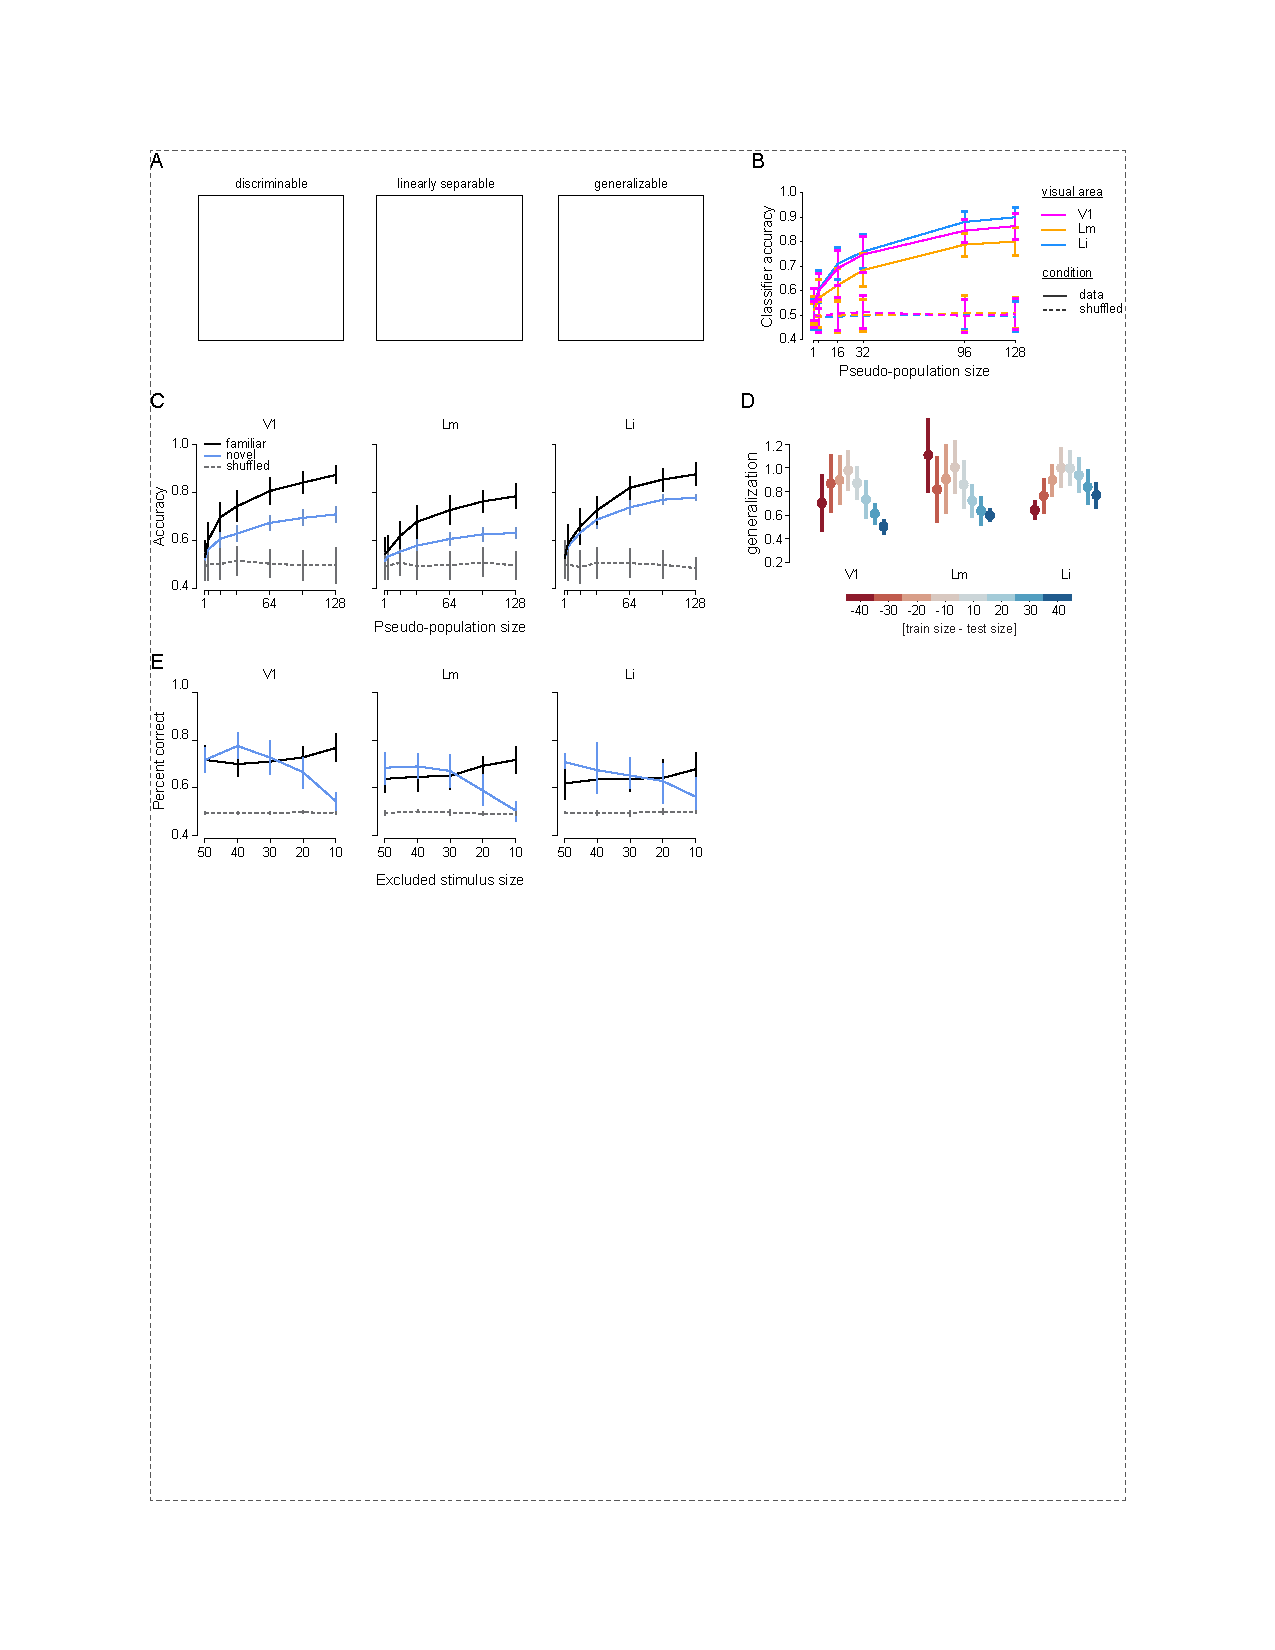
\includegraphics[width=\textwidth]{figures/chapter_4/fig_4-2_neural_generalization/fig_4-2_neural_generalization.pdf}
    \vspace{.1in}
    \caption[Population representations of objects]{Linear separability and generalization of population representations. 
    \textbf{A.} Schematic of tests for linear separability and generalization (adapted from \cite{Rust2010SelectivityIT}). \textit{Left}: A hypothetical population response for a single presentation of an image as a point in N-dimensional space, where N is the number of neurons in the population (illustrated here in 2D space, for 2 neurons). Different trials of the same image (blue dots) form a “cloud” in this N-dimensional space. The ability of the population to discriminate the different images is proportional to how far apart the response clouds are. Linear classifier approaches identify the optimal hyperplane that separates the responses to one image (blue cloud) from responses to all other images (green cloud). Performance on the discriminability task is measured as the proportion of times that response vectors on test trials correctly fall on the correct side of the hyperplane. \textit{Middle and Right}: Hypothetical representations that perform well or poorly under different tests of linear separability and tolerance. \textif{Middle}: A population that is linearly separable (black cloud separated from gray clouds) and could support generalization under one test (dashed line, “Trained on all conditions”) but fail under another (solid line, “Train on one condition,” and test on the others) with different views of a given object (blue clouds) assigned to the wrong side of the hyperplane. \textit{Right}: A population that is linearly separable and passes tests of generalization when testing on a single reference condition alone.
    \textbf{B.} Linear separability as a function of pseudo-population size (middle panel in \textbf{A}) for V1 (magenta), LM (orange), and LI (blue). Classifiers were trained on responses from all transformations simultaneously, then tested on a subset of trials not included in the training or cross-validation steps. Dotted lines indicate performance when object labels were shuffled. Error bars, bootstrapped estimates of the 95\% CI of the mean accuracy. 
    \textbf{C.} Tolerance as measured by classifier accuracy on generalization tests (right panel in \textbf{A}) as a function of pseudo-population size for V1 (left), LM (middle), and LI (right) populations. Populations were trained at a given stimulus size, then tested on new samples of the same stimulus size (black, “trained” stimulus size) and on samples of stimulus sizes not included in the training set (blue, “novel” stimulus sizes). Dotted lines indicate classifier accuracy when object labels were shuffled. Error bars, bootstrapped estimates of the 95\% CI of the mean accuracy.
    \textbf{D.} Generalization score for novel test conditions, split by the difference between train and test stimulus sizes. Generalization is defined as the ratio of classifier performance on novel conditions to performance on trained conditions (shown for the largest pseudo-population size tested, solid blue and black points at n=128 cells in \textbf{C}, but split by train-test combinations of stimulus size). Colors show stimulus size during training minus stimulus size during testing.
    \textbf{E.} Classifier performance on the generalization task as a function of training conditions for each imaging site (populations of simultaneously imaged cells). Classifiers were trained on the object identification task using a subset of 4 out of 5 stimulus sizes, then tested on different trials of the same stimulus size as training (black) and on trials of the held-out, untrained stimulus size (blue). Error bars show SD across imaging sites for each visual area. Dashed lines show performance when object labels were shuffled. 
    \label{fig:neural_generalization}}
\end{figure}


% Discussion. 

